% Start of Chapter 1 - System Analysis

An inverted pendulum is basically a consistent mass on the ground (usually wheeled), connected through a frictionless joint to a pendulum, so that the pendulum can freely rotate around the joint and fall down by its own weight. The goal in this system is to provide an horizontal force to the mass on the ground with a direction contrary to the inclination of the pendulum with respect to the vertical axis, so that the pendulum holds in its highest position.

\begin{figure}[h]
	\centering
	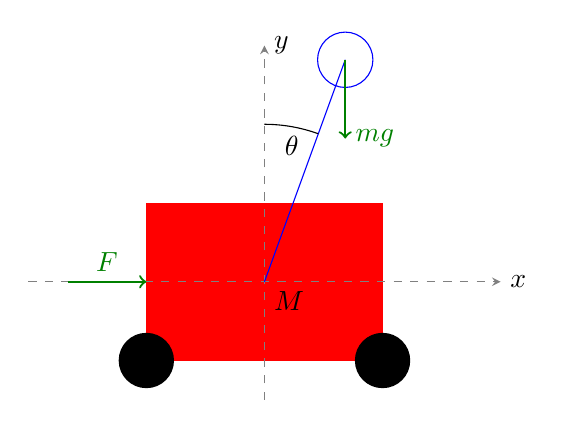
\begin{tikzpicture}
		% draw the red mass with two wheels
		\fill[red] (-1.5,-1) rectangle node[black, anchor=north west]{$M$} (1.5,1);
		\fill (-1.5,-1) circle [radius=10pt];
		\fill (1.5,-1) circle [radius=10pt];

		% draw the two coordinate axis
		\draw[dashed,>=stealth,->, draw=gray] (-3,0) -- (3,0) node[anchor=west]{$x$};
		\draw[dashed,>=stealth,->, draw=gray] (0,-1.5) -- (0,3) node[anchor=west]{$y$};

		% draw the pendulum
		\draw[blue] (0,0) -- ++(70:3) circle [fill=blue,radius=10pt];

		% draw the force of gravity in the pendulum
		\draw[green!50!black,->,thick] (70:3) -- +(0,-1) node[anchor=west]{$mg$};

		\draw[green!50!black,->,thick] (-2.5,0) -- node[anchor=south]{$F$} (-1.5,0);

		% draw the angle between pendulum and y-axis
		\draw (0,2) arc [start angle=90, end angle=70, radius=2] node[midway, below]{$\theta$};
	\end{tikzpicture}
	\caption{Physical representation of the inverted pendulum}\label{fig:diag}
\end{figure}

\section{Zumobot case study}

The case study in this work is based on a commercial Zumobot 32U4 (See figure \ref{fig:zumo}) robot from Pololu manufacturer. It consist on a rigid case that holds 2 brushless DC motors, an Arduino-compatible ATmega32U4 microcontroller and a set of batteries to power up the system. The motors are connected to a belt that rotates between to sets of wheels, sufficiently high to make the Zumobot able to stay in a vertical position without any contact between the case and the ground. The stucture is well suited for an inverted pendulum configuration, considering its physical characteristics and its simple programmability.

\begin{figure}[h]
	\centering
	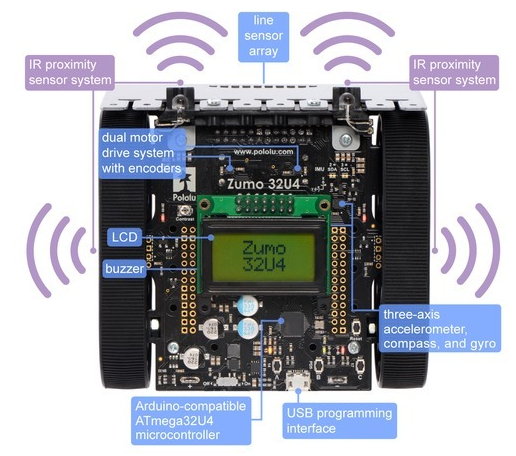
\includegraphics[scale=0.6]{zumo-superior.png}
	\caption{Pololu Zumobot}\label{fig:zumo}
\end{figure}

The goal position of the Zumobot is a vertical position with respect to the vertical axis. The Zumobot needs to be previously adjusted (frontal sensors holder dismounted), as the frontal part will face the ground, and the posterior part will be held up.

\begin{figure}[h]
	\centering
	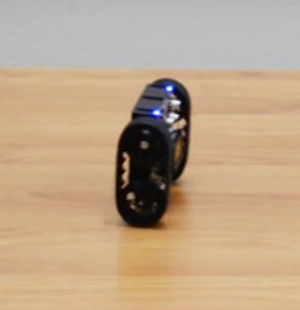
\includegraphics{zumo-balanced.png}
	\caption{Stabilized Zumobot position}\label{fig:zumoStable}
\end{figure}

The device includes several helpful sensors and peripherals:

\begin{itemize}
	\item AVR ATmega 32U4 microcontroller, with 16MHz crystal oscillator.
	\item Two micrometal gearmotors, driven by on-board TI DRV8838 motor divers.
	\item 3-axis accelerometer + 3-axis gyroscope
\end{itemize}

To power the motors, the microcontroller generates a PWM digital signal and a direction bit for each wheel (left and right). The Arduino environment provides a library to configure and control the PWM value with low effort. Along with the corresponding firmware, the whole actuator part of the system is complete.

The sensor part of the system uses the accelerometer and gyroscope to provide a value of the angle in the y axis, which is the axis that shows the angle $\theta$ defined in figure \ref{fig:diag}. The firmware in the Arduino controller gets the value from the gyroscope, and performs an adjustment of the value based on the accelerometer reading. It should be noted that the manufacturer of the robot states in the technical documentation\cite{POL01} that the accelerometer and gyroscope readings are likely to be influenced by external noise from the DC motors and the batteries, and the values obtained should only be considered for rough estimation.

\section{Control system}

The desired control system is then defined as shown in the figure \ref{fig:condiag}. It sets a desired reference of zero degrees, and provides a controller that calculates an appropiate control signal based on the error value to the plant.

\begin{figure}[h]
	\centering
	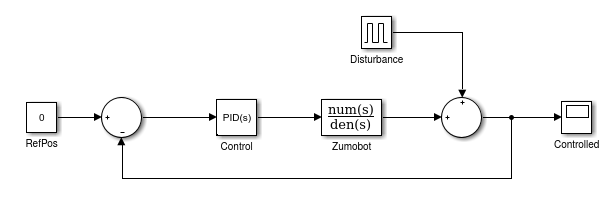
\includegraphics[scale=0.6]{control-system-simple.png}
	\caption{Control diagram of the inverted pendulum}\label{fig:condiag}
\end{figure}

The dynamics of the system can be divided into the following elements:
\begin{itemize}
	\item DC motor behavior to convert a DC voltage to a force
	\item Robot behavior defined by the physical characteristics
\end{itemize}

With this clarification, the control diagram of the system becomes as shown in figure \ref{fig:condiag2}.

\begin{figure}[h]
	\centering
	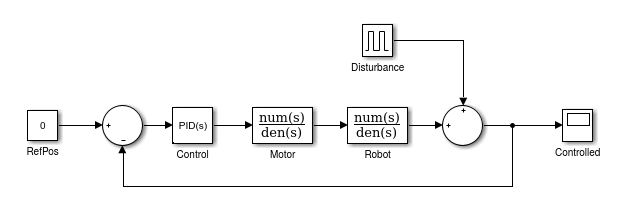
\includegraphics[scale=0.6]{control-system.png}
	\caption{Control diagram of the inverted pendulum - analysis elements}\label{fig:condiag2}
\end{figure}

To design the controller for the system, the dynamics of the motor and robot need to be defined. This is done in the next chapter by two different approaches.
